\documentclass{article} % For LaTeX2e
\usepackage{nips13submit_09,times}

\usepackage{hyperref}
\usepackage{url}
\usepackage{graphicx}
\usepackage{epstopdf}
\usepackage{multirow}
\usepackage{tabularx}
%\usepackage{adjustbox}


\title{CSE221 Operating System Measurement}

\author{
  Boyuan Qin\\
  \texttt{bqin@eng.ucsd.edu}\\
  \And
  Dexin Qi\\
  \texttt{deqi@eng.ucsd.edu}\\
  \And
  Qiheng Wang\\
  \texttt{qiw018@eng.ucsd.edu}\\
}
\date{\today}


\newcommand{\fix}{\marginpar{FIX}}
\newcommand{\new}{\marginpar{NEW}}

\nipsfinalcopy % Uncomment for camera-ready version

\begin{document}

\maketitle

\section{Introduction}
The goal of this project is to measure the performance of the operating
system, Ubuntu 12.04.4 LTS\@.  The reason behind this goal is to gain an
understanding of the relationship between the underlying hardware and the
operating system, and their effects on how much time integral operations will
require.  With this goal, we will be running a series of justified experiments
that will allow us to characterize the speed of each operation and compare
them to each other.  We will use the course of these experiments as a way of
gauging our intuition about the performance of the operating system we are
testing.  The information we will obtain from these experiments will also be
used in future endeavors as a set of performance results to compare against.

The language of choice in these tests will be C++.  The reason for choosing
C++ comes from the flexibility that C++ provides.  It is a high-level language
that allows us to, at the same time, work without much overhead as, for
example, Java when measuring time.  The compiler we are using is GCC
4.6.3-1ubuntu5 with no optimization.

The first part of the project required around 20 hours of work to complete. This included creating the tools necessary to measure the operating system and writing the report.

The experiments were split accordingly:

Measurement Overhead - Boyuan

Procedure Call Overhead - Dexin

System Call Overhead - Boyuan/Qiheng

Task Creation Time - Dexin

Context Switch Time -

\section{Machine Description}

The machine we used as the subject of our experiments is described in Table 1.

\begin{table}[h]
  \caption{Machine Specifications}
  \begin{center}
  \resizebox{\columnwidth}{!}{
  \begin{tabular}{|>{\centering\arraybackslash\bfseries}m{1in}|l|l|}
	\hline
	\multirow{8}{*}{Processor}          & Model                    & Intel\textregistered Core\texttrademark 2 Duo Processor P8600  \\ \cline{2-3}
	& Instruction Set                   & 64 bit                                                         \\ \cline{2-3}
	& Cycle Time                        & 0.417ns(2.4GHz frequency)                                      \\ \cline{2-3}
	& L1 data cache                     & 32KB per core, 8-way set associative, 64-byte line size        \\ \cline{2-3}
	& L1 instruction cache              & 32KB per, core 8-way set associative, 64-byte line size        \\ \cline{2-3}
	& L2 data cache                     & 3072KB, 12-way set associative, 64-byte line size              \\ \cline{2-3}
	& FSB                               & 1066 MHz                                                       \\
	\hline
	\multirow{11}{*}{Hard Drive}        & Model                    & Seagate Momentus\textregistered  5400.6 SATA model ST9500325AS \\ \cline{2-3}
	& Capacity                          & 500GB                                                          \\ \cline{2-3}
	& Cache                             & 8 Mbytes                                                       \\ \cline{2-3}
	& RPM                               & 5400                                                           \\ \cline{2-3}
	& Physical heads                    & 4                                                              \\ \cline{2-3}
	& Discs                             & 2                                                              \\ \cline{2-3}
	& Average Seek Read                 & 14ms typical                                                   \\ \cline{2-3}
	& Full Stroke Seek                  & 30ms                                                           \\ \cline{2-3}
	& Average Latency                   & 5.6ms                                                          \\ \cline{2-3}
	& Track to track seek time          & 1ms typical                                                    \\ \cline{2-3}
	& I/O data transfer rate            & 300 Mbytes/s max                                               \\
	\hline
	\multirow{3}{*}{Memory}             & Capacity                 & Dual channel(symetric), each 1024 MBytes                       \\ \cline{2-3}
	                                    & Frequency                & DDR3 PC3-10700 667 MHz                                         \\ \cline{2-3}
	                                    & Width                    & 64 bit per channel                                             \\
	\hline
	\multirow{2}{*}{Network Card}       & Model                    & Intel Wifi Link 5100                                           \\ \cline{2-3}
	                                    & Data Transfer Rate       & 300Mbps                                                        \\
	\hline
	\multicolumn{1}{|>{\bfseries}c|}{\multirow{2}{*}{OS}}   & \multirow{2}{*}{ Linux Distribution }       & Ubuntu 12.04.4 LTS               \\
	                                                        & \multicolumn{1}{c|}{}                       & GNU/Linux 3.8.0-35-generic i686 \\
	% here if use |c| instead of c|, will generate an extra vertical line
	\hline
  \end{tabular}
} % end of resizebox
  \end{center}
  \label{table:machine_description}
\end{table}


\section{CPU, Scheduling, and OS Services}

\subsection{Measurement Overhead}
The goal of this section is to report the overhead of reading system time and
the overhead of using loops to measure iterations of an operation.  These
measurements are important and necessary for accuracy of future experiments.

\subsubsection{Experiment Methodology}
we used and modified the \texttt{cycle.h} package from FFTW\cite{FFTW}.  The
\texttt{cycle.h} is a superset of the rdtsc which optimizes according to
different machines.  To read the time stamp counter, use \texttt{getticks()}
function. To calculate the difference of two time stamp, use \texttt{elapsed}
function, which returns a double precision value.  To measure the overhead
time for reading time, we simply executed \texttt{getticks()} twice in a row
and took the difference. The idea behind this methodology was to start
tracking immediately before the the execution of the next command and stop
tracking as soon as the command is executed. The difference between the two
\texttt{getticks()} times will give us the number of ticks taken between the
two methods. Similarly, measuring \texttt{elapsed()} required that we add two
\texttt{getticks()}, one before and one after, the \texttt{elapsed()} method.
We then determined the difference between the two \texttt{getticks()} methods
that preceded and followed the \texttt{elapsed()} method. Taking that
difference, we subtracted the time taken for one \texttt{getticks()} method to
account for the time necessary to execute the succeeding \texttt{getticks()}
to arrive at our final result.

To measure the overhead time for using a single loop, we chose to measure
a \texttt{for} loop that will increment a variable from 0 to 10000, and
divided it by 10000 to obtain the overhead taken by a single iteration, which
includes incrementing and checking. In order to measure purely the looping
part of the \texttt{for} loop, we put the variable declaration before the
first \texttt{getticks()} method. This way, we measured the time taken by the
loop to check and increment the variable. We also took into account the time
taken by the \texttt{getticks()} method and subtracted it from our final time.
Our motive behind choosing to test the \texttt{for} loop comes from our own foresight
of using \texttt{for} loops plentifully in future tests.

Each test was ran 10000 iterations, the mean was taken.  Each experiment was
ran 100 times, and the average and standard deviation were taken.

In order to accurately translate "ticks" into human time, a preliminary
measurement of the correlation is made between ticks and number of cycles is
1 to 1.  Since each cycle takes 0.416 ns, given our CPU frequency, we can make
the correlation that 1 tick is equivalent to 0.416 ns.
\subsubsection{Prediction}
We originally predicted that, for \texttt{getticks()}, the operation should be
less than 20 instructions. Assume CPI is 1, it would take the hardware less
than 20 cycles to finish this instruction. And elapsed should take a little
more time to execute since it has subtraction, while \texttt{getticks()} is
simply reading data. Since the OS has to manage procedure call and returning
values, we think software overhead should be less than 5 cycles.

For \texttt{for()} loop, with one arithmetic operation, one comparison and one
jump, it should take about 3 cycles. The OS will have to initialize the loop
counter, which should be less than 2 cycles.

\subsubsection{Experiment Results}

The experimental results are presented in Table~\ref{table:rdtsc_overhead}.

\begin{table}
  \caption{Reading overhead performance (in cycles)}
  \begin{tabular}{|l|l|l|l|l|l|}
    \hline
    Operation             & Hardware Est.         & Software Est.         & Prediction            & Mean          & Std. Deviation     \\ \hline
    \texttt{getticks}     & \textless20 (8.3 ns)  & \textless5 (2.1 ns)   & \textless25 (10.4 ns) & 45 (18.5 ns)  & \textasciitilde    \\ \hline
    \texttt{elapsed}      & \textless25 (10.4 ns) & \textless5 (2.1 ns)   & \textless30 (12.5 ns) & 36 (14.4 ns)  & \textasciitilde    \\ \hline
    \texttt{for} loop     & 3 (1.2 ns)            & 2 (0.8 ns)            & 5 (2.0 ns)            & 7 (2.8 ns)    & \textasciitilde    \\ \hline
  \end{tabular}
\label{table:rdtsc_overhead}
\end{table}
\subsubsection{Result Discussion}

The predicted performance was less than the measured performance. Our
predicted performance was based on the naive assumption that one task, such as
a jump, would only take 1 cycle to perform. However, looking at the measured
operation times, our assumption was proven to be false. This means that the
operating system and hardware were taking more cycles to perform each task.
A possible reason is that the compiler translate one line of code into several
instructions. Another reason might be CPU scheduling and context switching
between processes.

To note, both \texttt{getticks()} and \texttt{elapsed()} functions are
modified to be of inline attribute. Therefore, the measurement would eliminate
the overhead of procedual calls. On the other hand, the measured operation
time was close to the predicted operation time for the \texttt{for()} loop.
The difference here resided in our overlooking one or two operations while
making our prediction.

Our methodology centered around measuring the simplest possible operation for
reading time and for looping. Because we measured time immediately before and
immediately after the operation of interest, we successfully captured the
entirety of the operation. With this information, we will be able to use it as
a base from which we can accurately measure other performances.

\subsection{Procedure Call Overhead}
The goal of this section is to report the overhead of making a procedure call
with arguments. The number of arguments the procedure takes in will also be
taken into account in a series of tests. Each test will take in different
amounts of arguments ranging from 0 arguments to 7 arguments. These
measurements are important and necessary for accuracy of future experiments.

\subsubsection{Experiment Methodology}
To measure the overhead time of a procedure call, we measured the time to make
a call to a procedure that takes in the parameters given and does not
processing thereafter. The procedure itself does not return anything either.
In order to take into account the different time costs as a result of varying
amounts of parameters, we made procedure calls with 0 to 7 parameters. Each
procedure call with different amounts of parameters was tested 1000, and the
average and standard deviation were taken. Each procedure call was precluded
and succeeded by two different \texttt{getticks()}. Because of this, we also
took into account the amount of overhead \texttt{getticks()} populated and
subtracted that from the total in each procedure call.

Each of the procedure call did no processing of its arguments nor did it have
a return statement. The decision to make the procedure call in this way was
motivated by our goal of obtaining purely the overhead of making the call to
a procedure. It was decided that return statements and any processing of data
would not be part of the procedure call itself, and thus not included as part
of the testing processes.

\subsubsection{Prediction}
The number of parameter and size of parameter should both affect the time it
take for a processor call. Without parameters, a procedure should simply be two
jump instructions. Thus, we predict that the hardware cost of procedure call
with no parameters should be about 2. The OS need to remember where the
processor is called so that it can return, which should only take 1 cycle. As
parameter size grow, the OS will need to do more operations to copy the
parameters.

\subsubsection{Experiment Results}

\begin{figure}[!htb]
\centering
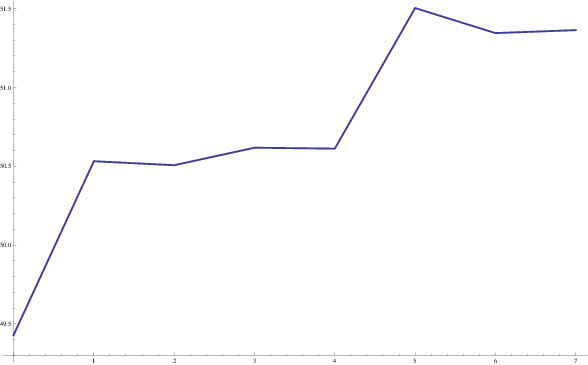
\includegraphics[scale=.6]{proc.png}
\caption{Procedure call performance (reading overhead included)}
\label{fig:proc}
\end{figure}

\subsubsection{Result Discussion}
An interesting discovery is that, the relationship between number of
parameters and the time to issue a procedure call is not a strict linear
relation. That indicates that, the OS is able to copy multiple
parameters(integer) in one cycle, which resulst in such a measurement result.
It appears that, every 4 integer parameters added will add one extra cycle of
overhead of a procedure call. Thus, we can get to the conclusion that the os
is able to copy 128 bits of data at the same time.

Notice that we did not substract the reading overhead in the graph, so the
actual overhead of procedure call should be 4~6 cycles. Thus, the overhead of
a procedure call is quite small. If the parameter size is large it will add to
the overhead, but still pretty fast.

\subsection{System Call Overhead}
The goal of this section is to report the overhead of making a system call and
compare it to the cost of making a procedure call. The system call with the
least overhead was chosen to accurately capture the time taken to make the the
switch from user mode to kernel mode. These measurements are important and
necessary for accuracy of future experiments.

\subsubsection{Experiment Methodology}
To measure the overhead time of a system call, we attempted to choose a method
with as little overhead as possible. Initially, our goal was to used
\texttt{getpid()} as our system call of choice. However, due to the potential
problem of having the \texttt{getpid()} system call getting cached and thus
not having an accurate overhead time of trapping into the kernel space, we
decided to choose a similar method, \texttt{getppid()}. In order to measure
the time of \texttt{getppid()}, we went about by simply adding
\texttt{getticks()} before and after the system call and calculated the
average difference and its standard deviation over 10000 runs. This method was
similar to the methodology described earlier in measuring loop overhead. We
then compared the results that we received to the results we measured earlier
for procedure calls.

\subsubsection{Experiment Results}

\subsubsection{Result Discussion}

\subsection{Task Creation Time}
The goal of this section is to report the time taken to create and run both
a process and a kernel thread, and to compare the two time costs.

\subsubsection{Experiment Methodology}
In order to measure time taken to create and run both a process and a kernel
thread, we used the basic principle of precluding and succeeding the target
section of code as we have prior. In order to create a kernel thread, we used
the method \texttt{pthread\_create()} to create and run a thread.

\texttt{pthread} allows us to avoid having to write kernel code and this
flexibility was one of the reasons why we decided to use it. The other reason
is that the thread is created executing any argument given as part of its
parameter. This means that we will not need to explicitly call any end
operation on the thread.

The arguments given to the \texttt{pthread\_create()} method were defaulted as
to avoid overhead that is separate from the task creation and minimal amount
of running. This test was repeated 10000 times, and the average and standard
deviation were taken while taking into consideration the overhead of reading
time. We used the same procedures for processes. We created processes using
\texttt{fork()} and terminated each process using \texttt{\_exit()}
immediately after creation and running.  Each experiment has 10000 iterations,
we run 100 experiments for process creation, and 1000 for thread
creation(since process creation is too slow) and the average and standard
deviation were taken while taking into consideration the overhead of reading
time.

\subsubsection{Prediction}
The time needed to create a task is really difficult to predict, since it
really dependents on how OS define a task, which means details such as process
data structure, thread data structure, implementation algorithms, will all
affect the time. Since we have little knowledge of linux kernel, we don't
think we can make a reasonable guess. One thing we would expect is that, the
time to create a process should be longer than creating a thread, since
processes are more heavy weighted than thread.

\subsubsection{Experiment Results}
\begin{table}[h]
  \begin{center}
    \caption{Thread creation performance (reading time included)}
    \begin{tabular}{|l|l|l|}
      \hline
      operation            & Mean of experiments       & Standard deviation       \\ \hline
      create process       & 209194.13(87.02 microsec) & 28245.38(11.75 microsec) \\ \hline
      create kernel thread & 3030.83(1.25 microsec)    & 68.57(28.53 ns)          \\ \hline
    \end{tabular}
    \label{table:thread_creating_results}
  \end{center}
\end{table}


\subsubsection{Result Discussion}
From the result, we could observe a significant difference between the time it
took to create a process and a kernel thread. We believe it is because
processes have much more complicated structure than threads. For example,
threads share memory while processes have separate address spaces. Such
a difference is reasonable in the sense that, threads are the minimum unit of
scheduling, and processes take advantage of threads to get better performance.
One more thing to mention, we actually measured the time it take for a kernel
module to create a kthread, and it seems to be even more time consuming than
process creation. We are wondering why would that happen, since a kernel
module is already in kernel level, it won't need to cross the boundary of user
level and kernel level again, why would it take so much time? Not to mention
it is a thread not a process.


\subsection{Context Switch Time}
The goal of this section is to report the time taken to context switch from
one process to another in comparison to the time taken to context switch from
one kernel thread to another.
\subsubsection{Experiment Methodology}
\subsubsection{Prediction}
\subsubsection{Experiment Results}
\subsubsection{Result Discussion}


\subsection{Time Consumption}
\subsubsection{CPU, Scheduling, and OS Services}
Boyuan Qin:\\
Dexin Qi: 22+ hours\\
Qiheng Wang:\\

\subsection{References}
http://en.wikipedia.org/wiki/Penryn\_(microprocessor)\\
http://tuxthink.blogspot.com/2011/02/kernel-thread-creation-1.html\\
http://jahanzebnotes.blogspot.com/2013/02/turn-off-cpu-throttling-ubuntu.html\\
http://www.seagate.com/staticfiles/support/disc/manuals/notebook/momentus/5400.6\%20(Wyatt)/100528359e.pdf\\
http://www.cpuid.com/softwares/cpu-z.html\\

%-----------------------------------------------------------------------------
% BIBLIOGRAPHY
%-----------------------------------------------------------------------------
\begin{thebibliography}{1}

\bibitem{FFTW} Cycle Counters. Available at {\tt http://www.fftw.org/download.html}.

\end{thebibliography}

\end{document}
